
\def\pagenum{1}
\def\vol{1}
\def\issue{1}

% ----------------------------- %
\documentclass[12pt]{article}

\usepackage[utf8]{inputenc} % Caracteres UTF-8
\usepackage[T1]{fontenc}
\usepackage[spanish]{babel} % Idioma español


\usepackage{times}                                     

\usepackage{FiraMono}
\renewcommand{\ttdefault}{fvm}
\DeclareTextFontCommand{\texttt}{\footnotesize\ttfamily}
\usepackage{minted}
\usemintedstyle{emacs}
\setminted{
  fontfamily=fvm, % FiraMono
  linenos,
  frame=lines,
  framesep=2mm,
  baselinestretch=1.2,
  fontsize=\footnotesize,
  breaklines=true,
  tabsize=4,
  numbersep=5pt,
  xleftmargin=1.5em,
  xrightmargin=1.5em
}
\setmintedinline{breaklines}


\usepackage{amsfonts,amsmath,amssymb, amsthm} 


\usepackage{latexsym}
\usepackage[letterpaper]{geometry}    

\usepackage{fancyhdr}
\usepackage{placeins}                           
\usepackage{xcolor}
\usepackage{graphicx}
\usepackage{tabularx}
\usepackage{array}



% Book Tables
\usepackage{booktabs}



\usepackage{comment}

% USE THIS TO CHANGE THE SPACING BETWEEN TABLES AND CAPTIONS!!!
\usepackage[labelfont=bf,labelsep=period, skip=5pt]{caption}
 

% TiKz
\usepackage{pgf,tikz}
\usepackage{mathrsfs}
\usetikzlibrary{arrows}

% PDF Plots
\usepackage{pgfplots}
\pgfplotsset{width=7cm,compat=1.10}

% For side-by-side figures
\usepackage{caption}
\usepackage{subcaption}
\usepackage{float}
\renewcommand{\topfraction}{0.9} % Máx. parte superior ocupada por floats
\renewcommand{\bottomfraction}{0.8} % Máx. parte inferior
\renewcommand{\textfraction}{0.1} % Mínimo texto que debe quedar
\renewcommand{\floatpagefraction}{0.8} % Requerido para página solo con floats



% Editing: highlight and strikethru
% \usepackage{soul}
% \usepackage{todonotes}  % editing (make comments \todo{X}
%\usepackage{lipsum}


% OUTLINES
\usepackage{outlines}
\usepackage{enumitem}
\setenumerate[1]{label=\arabic*.}
\setenumerate[2]{label=(\alph*).}
\setenumerate[3]{label=\roman*.}
\setenumerate[4]{label=\alph*.}

% Citations and References
% https://merkel.texture.rocks/Latex/natbib.php


% \makeatletter
% \renewcommand\@biblabel[1]{}
% \renewenvironment{thebibliography}[1]
%      {\section*{\refname}%
%       \@mkboth{\MakeUppercase\refname}{\MakeUppercase\refname}%
%       \list{}%
%            {\leftmargin0pt
%             \@openbib@code
%             \usecounter{enumiv}}%
%       \sloppy
%       \clubpenalty4000
%       \@clubpenalty \clubpenalty
%       \widowpenalty4000%
%       \sfcode`\.\@m}
%      {\def\@noitemerr
%        {\@latex@warning{Empty `thebibliography' environment}}%
%       \endlist}
% \makeatother




\RequirePackage{color}
\definecolor{cej@color}{rgb}{0.5,0.37109375,0.59765625}
\definecolor{abs}{rgb}{0.251,0.541,0.72.9}
\definecolor{ffqqqq}{rgb}{1,0,0}
\definecolor{qqqqff}{rgb}{0,0,1}
\definecolor{cqcqcq}{rgb}{0.75,0.75,0.75}
\definecolor{ttqqqq}{rgb}{0.2,0,0}
\definecolor{ffxfqq}{rgb}{1,0.5,0}
\definecolor{uuuuuu}{rgb}{0.27,0.27,0.27}
\definecolor{ffqqff}{rgb}{1,0,1}
\definecolor{xfqqff}{rgb}{0.5,0,1}
\definecolor{xdxdff}{rgb}{0.49,0.49,1}
\definecolor{red}{rgb}{1,0,0}
\definecolor{blue}{rgb}{0,0,1}
\definecolor{ccqqqq}{rgb}{0.8,0,0}
\definecolor{fftttt}{rgb}{1,0.2,0.2}
\definecolor{qqwuqq}{rgb}{0,0.39,0}
\definecolor{qqqqff}{rgb}{0,0,1}
\definecolor{wrwrwr}{rgb}{0.3803921568627451,0.3803921568627451,0.3803921568627451}
\definecolor{sexdts}{rgb}{0.1803921568627451,0.49019607843137253,0.19607843137254902}
\definecolor{rvwvcq}{rgb}{0.08235294117647059,0.396078431372549,0.7529411764705882}
\definecolor{ccqqqq}{rgb}{0.8,0,0}
\definecolor{qqqqff}{rgb}{0,0,1}
\definecolor{wwwwww}{rgb}{0.4,0.4,0.4}
\definecolor{qqwuqq}{rgb}{0,0.39215686274509803,0}
\definecolor{uuuuuu}{rgb}{0.266,0.266,0.266}

% Allows customization of titles
% \usepackage{titlesec}
% \titleformat{\section}[block]{\normalsize\scshape\bfseries{\arabic{section}.}}{}{1em}{}
% \titleformat{\section}[block]{\normalsize\scshape\bfseries}{\thesection}{1em}{}
% \titleformat*{\subsection}{\normalsize\scshape\itshape\bfseries}
% \titleformat*{\subsubsection}{\smallsize\scshape\itshape}

% \usepackage[hyphens]{url}
%\usepackage[hyphens,spaces,obeyspaces]{url}
% \usepackage[colorlinks,allcolors=blue]{hyperref}

\usepackage{titlesec}

\titleformat{\section}
  {\normalfont\fontsize{14}{14}\selectfont\bfseries} % 14pt, interlineado 16pt
  {\thesection.}{1em}{}

% Subsection con tamaño de 12pt
\titleformat{\subsection}
  {\normalfont\fontsize{12}{14}\selectfont\bfseries} % 12pt, interlineado 16pt
  {\thesubsection.}{1em}{}

% Subsubsection con tamaño de 10pt
\titleformat{\subsubsection}
  {\normalfont\fontsize{10}{12}\selectfont\bfseries} % 10pt, interlineado 16pt
  {\thesubsubsection.}{1em}{}

% Manejo de enlaces
\usepackage[colorlinks=true, linkcolor=black, citecolor=blue, urlcolor=blue]{hyperref}




\setcounter{page}{\pagenum}
\newcounter{ggbFirstpage}
\setcounter{ggbFirstpage}{\pagenum}
\pagestyle{empty}
\setlength{\headheight}{14pt}
\geometry{left=2cm,right=2cm,top=3cm,bottom=3cm}
\pagestyle{fancyplain}                              

\fancyhf{}
\fancyhead[c]{\small \emph{IE0523: Sistemas Digitales II, Proyecto final - Grupo 2}}     %
\cfoot{%                                            
  \ifnum\value{ggbFirstpage}=\pagenum%              
    {\vtop to\hsize{\hrule\vskip .2cm {\thepage}}}%   = the starting page number         %
  \else\setcounter{ggbFirstpage}{\pagenum}\fi%      
}                                                   

\newcommand*{\TitleFont}{%
      \usefont{\encodingdefault}{\rmdefault}{}{n}%
      \fontsize{16}{18}%
      \selectfont}

\def\authorfont{\normalfont\fontsize{12}{14}\selectfont\centering}
\def\subauthorfont{\normalfont\fontsize{10}{12}\selectfont\centering}
\definecolor{wrwrwr}{rgb}{0.3803921568627451,0.3803921568627451,0.3803921568627451}
\definecolor{sexdts}{rgb}{0.1803921568627451,0.49019607843137253,0.19607843137254902}
\definecolor{rvwvcq}{rgb}{0.08235294117647059,0.396078431372549,0.7529411764705882}
% \bibpunct[, ]{(}{)}{;}{a}{,}{,}


%\usepackage{mfirstuc}
% https://www.titlecase.com



 

\input{config/coding}
% ----------------------------- &


\usepackage{authblk}

\def\thetitle{\scshape{\textbf{Proyecto final IE-0523}}\\\vspace{0.25cm}Implementación de la subcapa de codificación física (PCS) según la cláusula 36 del estándar IEEE 802.3}

\def\authorOne{\authorfont{Daniel Alberto Sáenz Obando (C37099)},\\}
\def\authorTwo{\authorfont{Brandon Daniel Jiménez Campos (C33972)},\\}
\def\authorThree{\authorfont{Rodrigo Evelio Sánchez Araya (C37259)\\}}


\begin{document}

\interfootnotelinepenalty=100000

% ----------------------------- %
%  Header: Title, author
% ----------------------------- %
\title{\TitleFont{\thetitle}}
\author{\authorOne\authorTwo \vspace{0.45cm}\authorThree}


\vspace{-1mm}
\date{Escuela de Ingeniería Eléctrica, Universidad de Costa Rica\\\vspace{0.5cm}Fecha: 06-12-2025}
\maketitle



% ----------------------------- %
% Abstract
% ----------------------------- %
% abstract
%
\bgroup
\color{abs}
\hrule
\egroup



%
%%  DO NOT EDIT  LINES ABOVE                     %

\section{Resumen}

El presente documento expone el proyecto final del curso IE-0523 Sistemas Digitales II, cuyo objetivo principal consiste en la implementación en Verilog HDL de la subcapa de codificación física (\textit{Physical Coding Sublayer}, PCS) definida en la cláusula 36 del estándar IEEE 802.3 para el tipo 1000BASE-X.

El trabajo desarrollado aborda el análisis detallado del estándar, la descomposición funcional del PCS y el diseño modular de los bloques que conforman la etapa de transmisión (\texttt{TRANSMIT}), sincronización (\texttt{SYNCHRONIZATION}) y recepción (\texttt{RECEIVE}).
Se describen las estructuras arquitectónicas diseñadas, el comportamiento esperado de cada módulo, las señales relevantes y la metodología utilizada para el desarrollo de las pruebas y en el trabajo colaborativo.
Asimismo, se conectaron los tres módulos en modo \textit{loopback} para su prueba final.

El proyecto se basa en un esquema modular, donde se reutilizan componentes y convenciones comunes con el fin de asegurar cohesión y claridad en el desarrollo del código, tanto para el entendimiento del profesor al calificar como para los estudiantes durante la realización del proyecto.
El resultado más importante es que se tuvieron los resultados esperados según la cláusula del estándar dado, lo cual equivale a un proyecto exitoso.

\thispagestyle{fancy}


% ----------------------------- %
% Sections
% ----------------------------- %
\section{Medología}
Para garantizar coherencia, calidad y un buen trabajo en paralelo, se utilizó:

\begin{enumerate}[label=\textbf{\arabic*.}]
    \item \textbf{Formato de código estandarizado}
    
    \begin{itemize}
        \item Plantilla llamada \texttt{template.v} para tener una misma estructura.
        \item Uso de la herramienta \texttt{Verible} para formateo automático y consistencia de estilo en todo el código.
        \item Señales llamadas igual al estándar y en minúscula.
        \item Nombres de estados en mayúscula.
    \end{itemize}
    
    \item \textbf{Flujo de trabajo con GitHub}
    
    \begin{itemize}
        \item Desarrollo por \textit{branches} para funcionalidades aisladas.
        \item Manejo de tareas mediante \textit{issues}.
        \item Revisiones e integraciones de código mediante \textit{pull requests}.
    \end{itemize}
    
    \item \textbf{Repartición de módulos}
    
    \begin{itemize}
        \item Daniel Sáenz: Módulo Transmisor.
        \item Rodrigo Sánchez: Módulo Sincronizador.
        \item Brandon Jiménez: Módulo Receptor.
    \end{itemize}
\end{enumerate}
\section{Descripción arquitectónica}

Ahora bien, en cuanto a la arquitectura del sistema implementado en Verilog HDL, se tiene que la PCS consiste de 5 módulos: \texttt{TRANSMIT}, \texttt{RECEIVE}, \texttt{SYNCHRONIZATION}, \texttt{CARRIER-SENSE} y \texttt{AUTO-NEGOTIATION} \cite{IEEE8023-2018}.
Según los alcances establecidos en el enunciado del proyecto, se implementaron únicamente los tres primeros y se aseguró de que las señales manejadas por los otros módulos tuvieran el comportamiento esperado.

Entonces, a continuación se explican cada uno de los módulos, las señales de entrada y salida que los conforman, los estados seleccionados y el diagrama ASM que describe el comportamiento de la máquina de estados.

\subsection{Módulo \texttt{TRANSMIT}}

Respecto al submódulo de transmisión, este está dividido en dos máquinas de estado separadas: \textit{transmit code-group} y \textit{transmit ordered set}.
En la Figura \ref{fig:transmisor-diagrama_bloques}, se muestra un diagrama de bloques donde se indican las conexiones de las máquinas de estados.

\begin{figure}[htb]
    \centering
    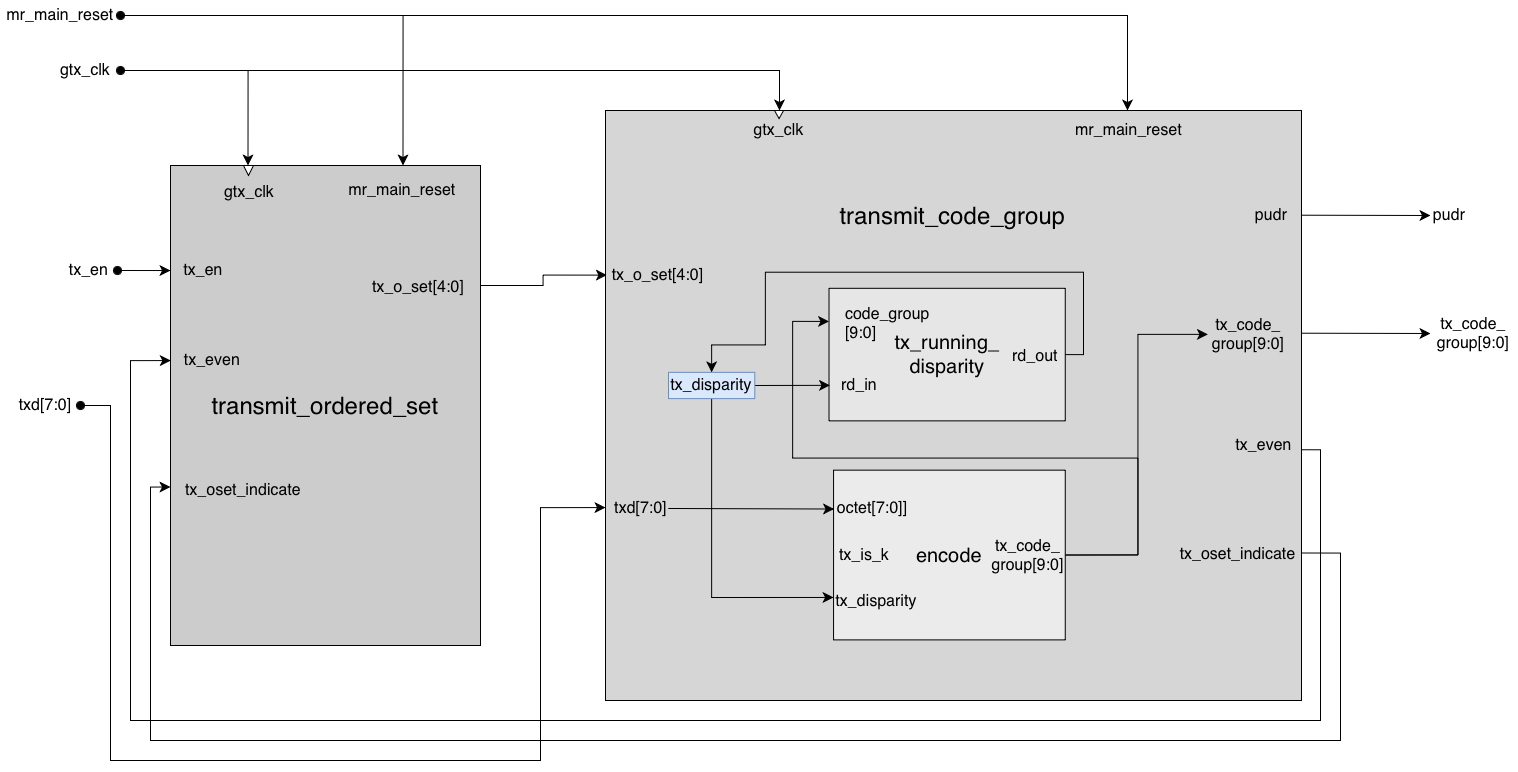
\includegraphics[width=\textwidth]{images/diagrama-bloques-transmisor.png}
    \caption{Diagrama de bloques del módulo \texttt{TRANSMIT}.}
    \label{fig:transmisor-diagrama_bloques}
\end{figure}

Antes de continuar con la explicación de las máquinas de estado principales, se van a explicar los bloques combinacionales \texttt{encode} y \texttt{running\_disparity} creados para facilitar el diseño.
El primero corresponde a un \textit{lookup table} que recibe el \texttt{running\_disparity} actual y la señal \texttt{txd} de 8 bits.
A partir de estos datos, coloca en su salida el \textit{code-group} resultante de 10 bits.

El segundo corresponde al módulo que recibe el \textit{code-group} actual junto con el \texttt{running\_disparity} actual y calcula el siguiente \texttt{running\_disparity}.
Por lo tanto, ambos módulos funcionan para modularizar el código de la máquina de estados \texttt{transmit\_code\_group} y facilita el diseño y mantenimiento del código.

Ahora sí, se continúa con la explicación de la arquitectura de las máquinas de estados principales.

\subsubsection{Submódulo \texttt{transmit\_code\_group}}

Inicialmente, se realiza una descripción del funcionamiento esperado de este bloque.
El módulo selecciona el octeto apropiado para transmisión, ya sea datos o alguno de los símbolos especiales \texttt{/S/}, \texttt{/T/}, \texttt{/R/} o \texttt{/I/}.
Además, determina si el símbolo corresponde a un carácter de tipo K mediante la señal \texttt{tx\_is\_k}, requerida para la codificación 8b/10b.
También actualiza la señal \texttt{tx\_even} con el fin de distinguir entre ciclos pares e impares.
Posteriormente, genera el code-group de 10 bits en \texttt{tx\_code\_group}.
Una vez que el code-group está listo, activa la señal \texttt{tx\_oset\_indicate} para informar al módulo \texttt{transmit\_ordered\_set}.
Finalmente, habilita la señal \texttt{pudr} cuando el code-group se encuentra disponible para ser enviado hacia la capa PMA.

En el estándar IEEE 802.3, se muestra un diagrama de estados complejo con estados repetidos y/o sobrantes, que no entran dentro del contexto del proyecto, ya sea por ser de manejo de errores o de configuración.
Estos fueron eliminados y los finales se muestran en la Figura \ref{fig:transmit_code_group_asm}.

\begin{figure}[htb]
    \centering
    
\includegraphics[width=0.8\textwidth]{images/transmit_code_group_asm.png}
    \caption{Diagrama ASM del módulo \texttt{transmit\_code\_group}.}
    \label{fig:transmit_code_group_asm}
\end{figure}

Para la codificación de los estados del diagrama ASM correspondiente, se utilizó \textit{one-hot encoding}.
Esta es fundamental para evitar condiciones de carrera en implementaciones reales.
Estos se muestran en el Cuadro \ref{tab:estados-transmit_code_group}.

\begin{table}[htb]
    \centering
    \begin{tabular}{cc}
    \hline
    \textbf{Estado} & \textbf{Codificación} \\
    \hline
    \texttt{GENERATE\_CODE\_GROUPS} & 2'b01 \\
    \texttt{IDLE\_2} & 2'b10 \\
    \hline
    \end{tabular}
    \caption{Estados del módulo \texttt{transmit\_code\_group}.}
    \label{tab:estados-transmit_code_group}
\end{table}

Para completar la descripción arquitectónica, en el Cuadro \ref{tab:transmit_code_group_senales}, se muestran las señales de entrada y salida del módulo \texttt{transmit\_code\_group}.
Así como una descripción del funcionamiento de la señal en cuestión.

\begin{table}[htb]
    \centering
    \begin{tabular}{lcp{7cm}}
    \hline
    \textbf{Señal} & \textbf{Tipo} & \textbf{Descripción} \\ \hline
    \texttt{gtx\_clk} & Entrada & Reloj de transmisión del bloque PCS. \\
    \texttt{mr\_main\_reset} & Entrada & Reinicio global del transmisor, activo en alto. \\
    \texttt{txd [OCTET\_WIDTH-1:0]} & Entrada & Octeto de datos a transmitir cuando \texttt{tx\_o\_set} indica \texttt{/D/}. \\
    \texttt{tx\_o\_set [TX\_O\_SET\_WIDTH-1:0]} & Entrada & Identificador del tipo de ordered set (\texttt{/I/}, \texttt{/S/}, \texttt{/D/}, \texttt{/T/}, \texttt{/R/}). \\
    \texttt{tx\_code\_group [CG\_WIDTH-1:0]} & Salida & Code-group que se envía hacia la capa PMA. \\
    \texttt{tx\_even} & Salida & Indicador de ciclo par/impar. \\
    \texttt{tx\_oset\_indicate} & Salida & Señal que indica que el code-group actual se encuentra listo para que \texttt{transmit\_ordered\_set} avance. \\
    \texttt{pudr} & Salida & Señal de indicación hacia la PMA de que existe un nuevo code-group disponible en \texttt{tx\_code\_group}. \\ \hline
    \end{tabular}
    \caption{Señales de entrada y salida de \texttt{transmit\_code\_group}.}
    \label{tab:transmit_code_group_senales}
\end{table}

\subsubsection{Submódulo \texttt{transmit\_ordered\_set}}

Respecto al módulo \texttt{transmit\_ordered\_set}, se tiene que este se encarga de generar el comportamiento descrito a continuación:
El módulo permanece en el estado \texttt{IDLE} (representado por \texttt{/I/}) cuando la transmisión no se encuentra habilitada.
Una vez que la señal \texttt{tx\_en} se activa, el módulo detecta el inicio de una trama y emite el símbolo \texttt{/S/} (\textit{Start of Packet}).
Posteriormente, transmite \texttt{/D/} mientras existan datos válidos disponibles.
Al finalizar la trama, genera el símbolo \texttt{/T/} y, según el valor de \texttt{tx\_even}, determina si es necesario aplicar \textit{carrier extend} mediante la emisión del símbolo \texttt{/R/}.

Adicionalmente, se muestra en la Figura \ref{fig:transmit_ordered_set_asm} el diagrama ASM simplificado del estándar IEEE 802.3, al igual que en el caso anterior.
Se simplificaron estados principalmente para coincidir con las temporaciones necesarias según los ciclos de reloj que debe tomar.
Para ello, se siguieron las indicaciones dadas por el profesor en clase.

\begin{figure}[htb]
    \centering
    
\includegraphics[width=0.45\textwidth]{images/transmit_ordered_set_asm.png}
    \caption{Diagrama ASM del módulo \texttt{transmit\_ordered\_set}.}
    \label{fig:transmit_ordered_set_asm}
\end{figure}

Los estados del diagrama ASM fueron codificados con \textit{one hot} y su código respectivo se muestra en el Cuadro \ref{tab:estados-transmit_ordered_set}.

\begin{table}[htb]
    \centering
    \begin{tabular}{cc}
    \hline
    \textbf{Estado} & \textbf{Codificación} \\
    \hline
    \texttt{XMIT\_DATA} & 3'b001 \\
    \texttt{TX\_PACKET} & 3'b010 \\
    \texttt{EPD} & 3'b100 \\
    \hline
    \end{tabular}
    \caption{Estados del módulo \texttt{transmit\_ordered\_set}.}
    \label{tab:estados-transmit_ordered_set}
\end{table}

Finalmente, las señales de entrada y salida de este submódulo, se indican en el Cuadro \ref{tab:transmit_ordered_set_senales}.
Adicionalmente, se agregó una breve descripción de lo que significan.

\begin{table}[H]
    \centering
    \begin{tabular}{lcp{7cm}}
    \hline
    \textbf{Señal} & \textbf{Tipo} & \textbf{Descripción} \\ 
    \hline
    \texttt{gtx\_clk} & Entrada & Reloj de transmisión del bloque PCS. \\
    \texttt{mr\_main\_reset} & Entrada & Reinicio global del transmisor, activo en alto. \\
    \texttt{tx\_even} & Entrada & Indicador de ciclo par/impar para decidir la aplicación de \textit{carrier extend}. \\
    \texttt{tx\_oset\_indicate} & Entrada & Señal que indica que el \textit{code group} actual ya se envió. \\
    \texttt{tx\_en} & Entrada & Habilitación de transmisión. \\
    \texttt{tx\_o\_set [TX\_O\_SET\_WIDTH-1:0]} & Salida & Identificador del ordered set a enviar (\texttt{/I/}, \texttt{/S/}, \texttt{/D/}, \texttt{/T/}, \texttt{/R/}). \\ \hline
    \end{tabular}
    \caption{Señales de entrada y salida de \texttt{transmit\_ordered\_set}.}
    \label{tab:transmit_ordered_set_senales}
\end{table}

\subsection{Módulo \texttt{SYNCHRONIZATION}}

En la Figura \ref{sincBlock} se muestra el diagrama de bloques estipulado para el módulo de \texttt{SYNCHRONIZATION}, con sus respectivas entradas y salidas.
El principal punto a destacar es la salida del \texttt{SUDI}, la cual en este caso es de 11 bits, donde los primeros 10 bits corresponden al code-group proveniente del \texttt{PUDI} y el último es el correspondiente a \texttt{rx\_even}.

\begin{figure}[H]
    \centering
    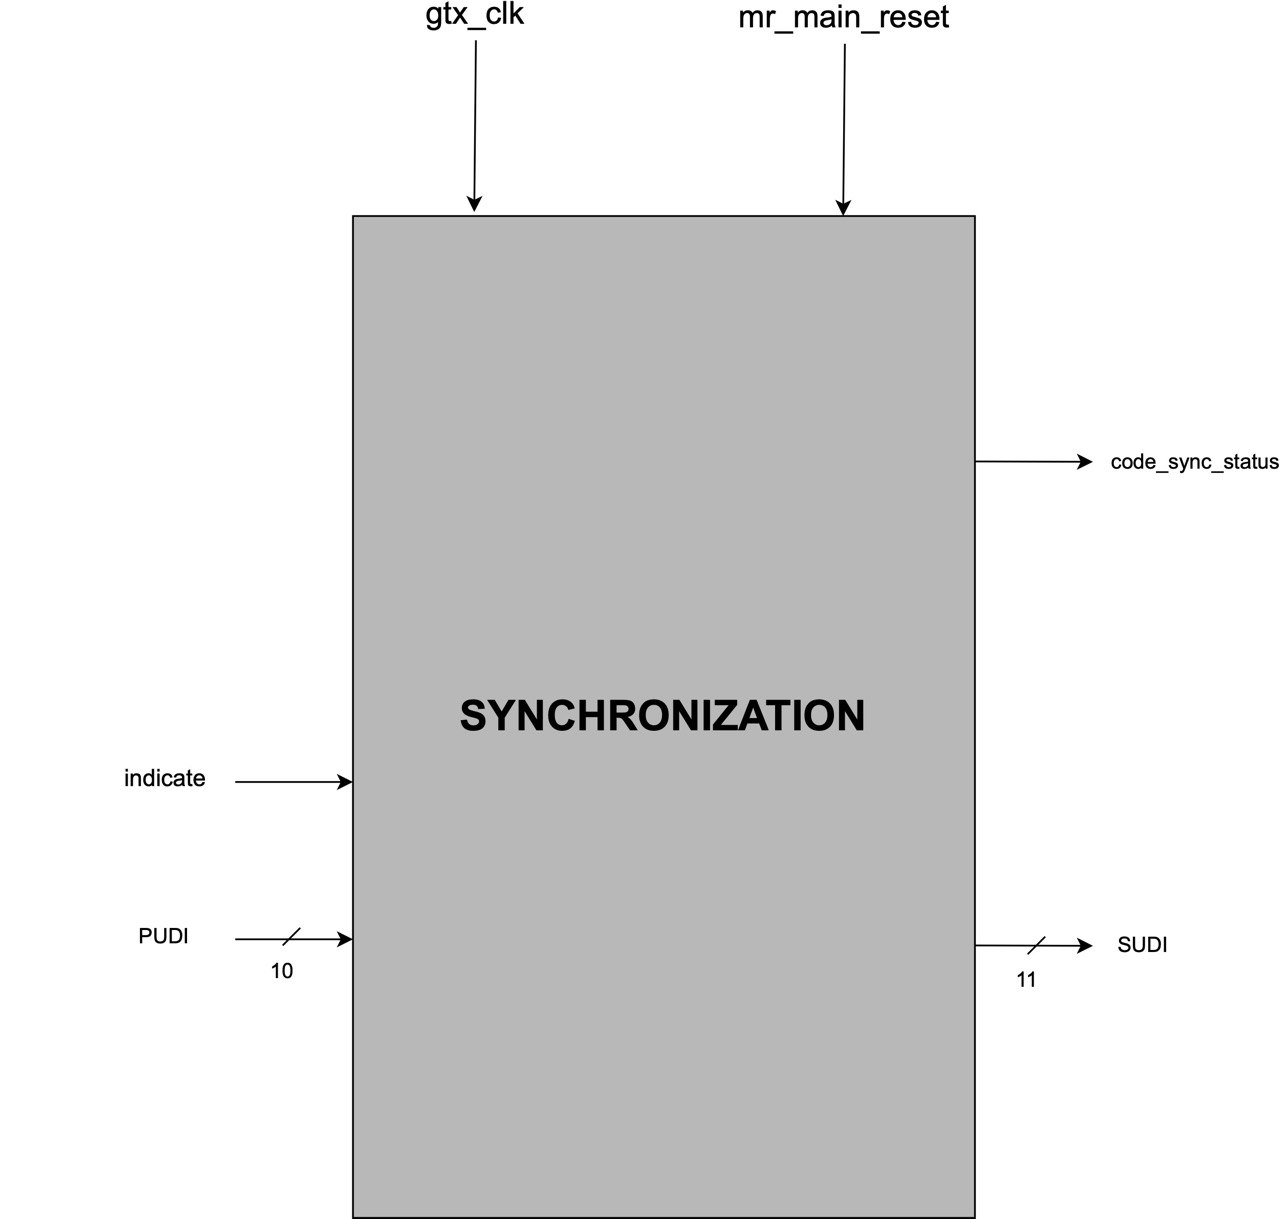
\includegraphics[width=0.6\textwidth]{images/sync_block.jpg}
    \caption{Diagrama de bloques del módulo \texttt{Synchronization}.}
    \label{sincBlock}
\end{figure}

Asimismo, dentro de este módulo, se tiene una instancia de \texttt{pudi\_checker}, que corresponde a un submódulo combinacional, que permite clasificar los \texttt{PUDI} recibidos en válidos/inválidos.

Para la sincronización inicial a partir del estado \texttt{LOSS\_OF\_SYNC}, se utilizaron contadores para ahorrar estados en este proceso.
Para el proceso de pérdida de sincronización, se mantuvo la estructura de estados mostrada en el estándar IEEE 802.3, con el fin de simplificar la programación, entendimiento y estructura del código.

En el Cuadro \ref{entradasysalidasSync} se observa con más detalle las entradas y salidas del módulo de \texttt{SYNCHRONIZATION}. 
Además, en el Cuadro \ref{estadosSync} se muestran los estados referentes al presente módulo, junto con una breve descripción de lo que hace cada uno. 

\begin{table}[htb]
\centering
\begin{tabular}{lcp{7cm}}
\hline
\textbf{Señal} & \textbf{Tipo} & \textbf{Descripción} \\ \hline
\texttt{mr\_main\_reset} & Entrada &   Reset activo en alto. Inicializa el sistema y fuerza el estado IDLE. \\
\texttt{clk} & Entrada & Señal de reloj principal del sistema. \\
\texttt{indicate} & Entrada & Indica que hay un code-group recibido. Proviene de la señal PUDR del transmisor (en \textit{loopback}). \\
\texttt{PUDI[CG\_WIDTH-1:0]} & Entrada & Code-group recibido desde el PMA. \\
\texttt{code\_sync\_status} & Salida & Indica sincronización adquirida. \\
\texttt{SUDI[CG\_WIDTH:0]} & Salida &  Code-group extendido a 11 bits (PUDI + rx\_even). \\ \hline
\end{tabular}
\caption{Señales de entrada y salida del módulo \texttt{SYNCHRONIZATION}.}
\label{entradasysalidasSync}
\end{table}

\begin{table}[H]
    \centering
    \begin{tabular}{ccp{7cm}}
    \hline
    \textbf{Estado} & \textbf{Código} & \textbf{Descripción} \\ \hline
    \texttt{LOSS\_OF\_SYNC} & 10'b0000000001 & Indica pérdida de sincronización. Se espera la aparición de una comma /K28.5/ válida. \\
    \texttt{COMMA\_DETECT} & 10'b0000000010 & Se detecta la comma por primera vez. Verifica que el siguiente code-group sea un D válido. \\
    \texttt{ACQUIRE\_SYNC} & 10'b0000000100 & Se detecta un dato válido, espera a que se lleguen a dos commas y dos datos para estar sincronizado. \\
    \texttt{SYNC\_ACQUIRED\_1} & 10'b0000001000 & Primer nivel de sincronización establecida. \texttt{rx\_even} alterna y se valida la calidad de los code-groups. \\
    \texttt{SYNC\_ACQUIRED\_2} & 10'b0000010000 & Un error detectado. Espera un code-group válido para volver a sincronizarse o uno inválido para seguir perdiendo sincronía. \\
    \texttt{SYNC\_ACQUIRED\_2A} & 10'b0010000000 & Se detectó un code-group válido después del primer inválido. Requiere 3 válidos para volver a estar sincronizado totalmente. \\
    \texttt{SYNC\_ACQUIRED\_3} & 10'b0000100000 & Dos code-groups inválidos. Mismo funcionamiento que \texttt{SYNC\_ACQUIRED\_2}. \\
    \texttt{SYNC\_ACQUIRED\_3A} & 10'b0100000000 & Mismo funcionamiento que \texttt{SYNC\_ACQUIRED\_2A}, pero para dos code-groups inválidos detectados. \\
    \texttt{SYNC\_ACQUIRED\_4} & 10'b0001000000 & Tres code-groups inválidos. \\
    \texttt{SYNC\_ACQUIRED\_4A} & 10'b1000000000 & Mismo funcionamiento que \texttt{SYNC\_ACQUIRED\_2A}, pero para tres code-groups inválidos. \\ \hline
    \end{tabular}
    \caption{Estados del módulo \texttt{SYNCHRONIZATION}.}
    \label{estadosSync}
\end{table}

Por último, se muestra el diagrama de estados ASM planteado para el módulo de \texttt{SYNCHRONIZATION} en la Figura \ref{asmSync}. 

\begin{figure}[H]
    \centering
    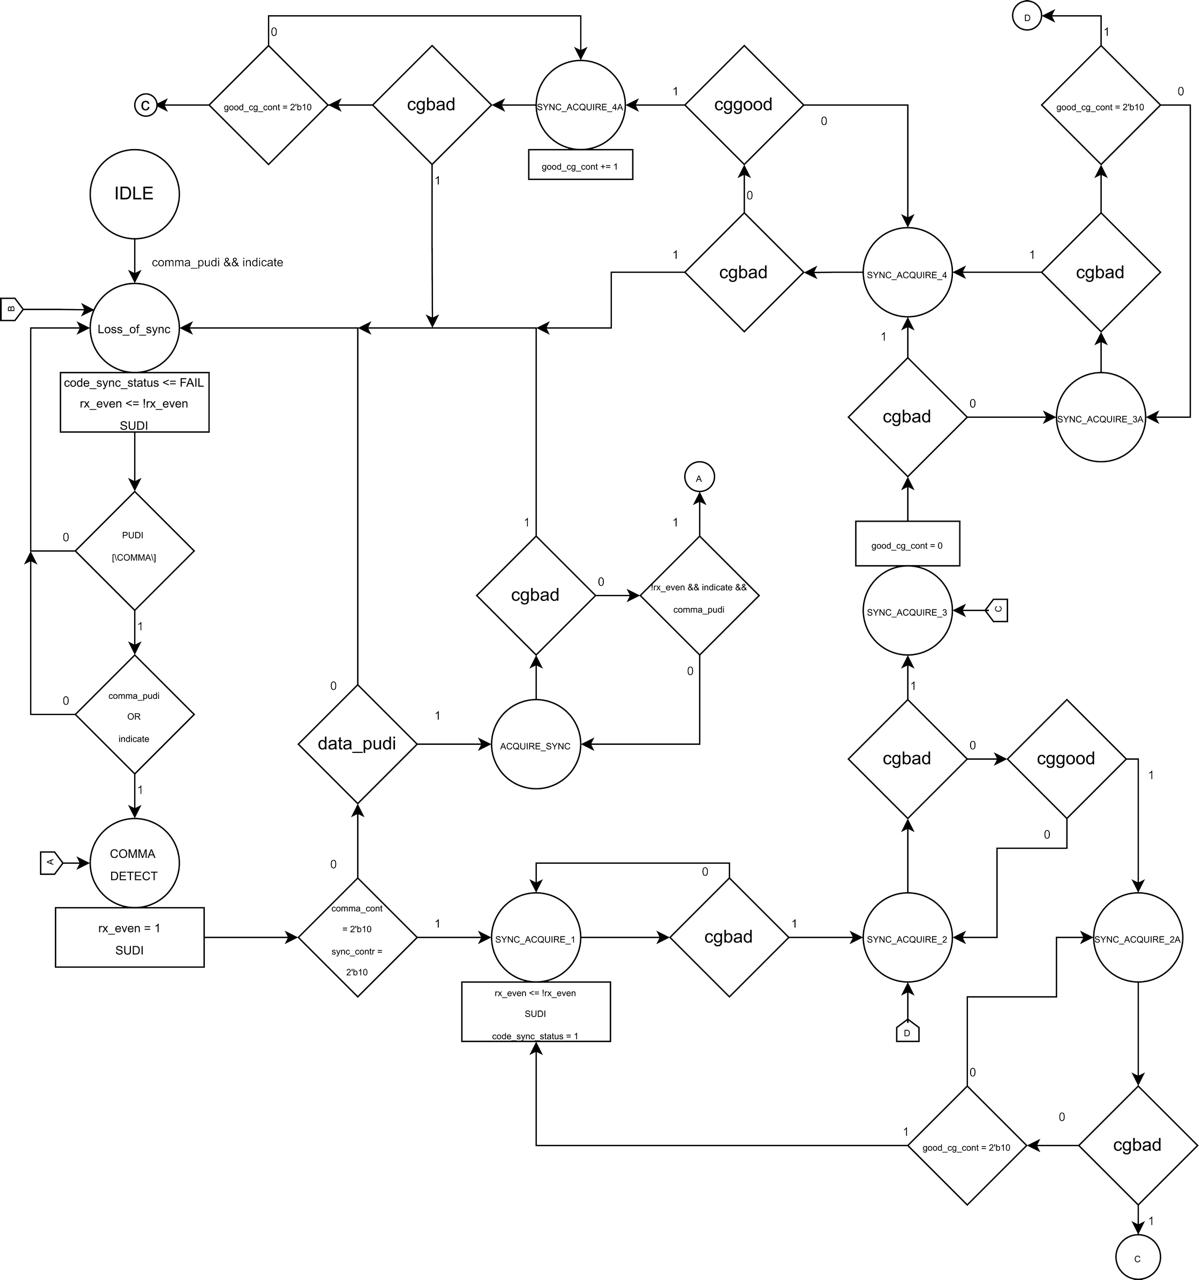
\includegraphics[width=\textwidth]{images/synchronization_ASM.jpg}
    \caption{Diagrama ASM del módulo \texttt{SYNCHRONIZATION}.}
    \label{asmSync}
\end{figure}


\subsection{Módulo \texttt{RECEIVE}}

Para el módulo de recepción, se trabajó instanciando 2 módulos, los cuales están dentro del módulo principal del receptor, tal y como se observa en la Figura \ref{receive_block}.
Se tiene un submódulo \texttt{running\_disparity}, el cual se encarga de calcular el próximo valor del running disparity según el running disparity actual y el \texttt{rx\_code\_group}.
Además, el módulo de \texttt{decode} se encarga de convertir de 10 bits a 8 bits el code-group recibido.
Este necesita el valor actual del running disparity y el \texttt{rx\_code\_group} para poder decodificar de manera correcta, y con esto se obtiene el valor del octeto y se envía a través de la salida \texttt{rxd}.

\begin{figure}[H]
    \centering
    
\includegraphics[width=\linewidth]{images/receive_block.png}
    \caption{Diagrama de bloques del módulo \texttt{RECEIVE}.}
    \label{receive_block}
\end{figure}

Las señales que están en el módulo de \texttt{RECEIVE} se observan en el Cuadro \ref{señales_receive}, donde se da una breve descripción de cada señal y su tipo.
\begin{table}[H]
    \centering
    \begin{tabular}{ccp{7cm}}
    \hline
    \textbf{Señal} & \textbf{Tipo} & \textbf{Descripción} \\
    \hline
    \texttt{rx\_clk} & Entrada & Reloj con el que funciona el receptor para el envio de datos. \\
    \texttt{mr\_main\_reset} & Entrada & Controla el reinicio de la PCS (activo en alto). \\
    \texttt{SUDI[10:0]} & Entrada & Señal enviada por el proceso de sincronización al proceso de recepción que contiene los bits del code-group y también el \texttt{rx\_even} (en el LSB). \\
    \texttt{sync\_status} & Entrada & Indica la sincronización (activo en alto). \\
    \texttt{rxd[7:0]} & Salida & Es el valor que entrega el receptor a la interfaz GMII. \\
    \texttt{rx\_dv} & Salida & Indica que los valores de \texttt{rxd} son válidos. \\
    \texttt{rx\_er} & Salida & Indica que los valores de \texttt{rxd} contienen un error. \\
    \hline
    \end{tabular}
    \caption{Señales del módulo \texttt{RECEIVE}.}
    \label{señales_receive}
\end{table}

\indent Además, se simplificaron los estados del módulo \texttt{RECEIVE}, pasando a tener 6 estados de 31 estados que contiene el estándar en el caso del receptor.
Además, para los estados implementados se utilizó la codificación \textit{one-hot}, estos se pueden observar en el Cuadro \ref{estados_receive}.

\begin{table}[H]
    \centering
    \begin{tabular}{cc}
    \hline
    \textbf{Estado} & \textbf{Codificación} \\
    \hline
    \texttt{LINK\_FAILED} & 6'b000001 \\
    \texttt{WAIT\_FOR\_K} & 6'b000010 \\
    \texttt{RX\_K} & 6'b000100 \\
    \texttt{IDLE\_D} & 6'b001000 \\
    \texttt{RECEIVE} & 6'b010000 \\
    \texttt{TRI\_RRI} & 6'b100000 \\
    \hline
    \end{tabular}
    \caption{Estados del módulo \texttt{RECEIVE}.}
    \label{estados_receive}
\end{table}

A continuación, en la Figura \ref{receive_asm} se presenta el diagrama ASM simplificado que se utilizó para el funcionamiento del módulo de \texttt{RECEIVE}.

\begin{figure}[H]
    \centering
    
\includegraphics[width=0.8\textwidth]{images/receive_asm.png}
    \caption{Diagrama ASM de la máquina de estados de \texttt{RECEIVE.}}
    \label{receive_asm}
\end{figure}

\section{Plan de pruebas}

En este apartado, se describen las pruebas desarrolladas para cada uno de los submódulos individuales, así como para el PCS completo que integra los tres submódulos.
Estas fueron implementadas para asegurar el correcto funcionamiento de las máquinas de estados separadas, así como en conjunto.
Se probó una variedad de casos para cada uno, donde se contempló el funcionamiento normal y algunas variaciones.

\subsection{Módulo \texttt{TRANSMIT}}

En esta subsección se describen las pruebas funcionales aplicadas al módulo de transmisión completo, utilizando el probador en \texttt{src/transmit/tester.v}.
Cada prueba define una secuencia de octetos de datos (\texttt{txd}) y una activación de la señal \texttt{tx\_en}, con el objetivo de verificar el comportamiento del transmisor respecto a:
\begin{itemize}
  \item La generación correcta de los \textit{ordered sets}: \texttt{/S/}, \texttt{/D/}, \texttt{/T/}, \texttt{/R/} e \texttt{/I/}.
  \item La presencia o ausencia de \textit{carrier extend} (\texttt{/R R/} después de \texttt{/T/}).
  \item El manejo del \textit{running disparity} y la selección del IDLE correcto (\texttt{/I1/} o \texttt{/I2/}).
\end{itemize}

A continuación se detalla cada una de las pruebas definidas.

\subsubsection*{Prueba 0: IDLEs después de \texttt{reset}}

\begin{itemize}
  \item \textbf{Descripción:} Tras el \texttt{reset}, se espera un período de inactividad donde \texttt{tx\_en = 0} y el transmisor permanece en estado de \texttt{IDLE}.
  \item \textbf{Resultado esperado:}
    \begin{itemize}
      \item El transmisor debe generar únicamente \textit{ordered sets} de tipo \texttt{/I/} (secuencias \texttt{/K28.5/} seguidas de \texttt{/D16.2/}.
      \item No deben aparecer símbolos de inicio de trama (\texttt{/S/}), datos (\texttt{/D/}), terminación (\texttt{/T/}) ni extendidos (\texttt{/R/}) mientras \texttt{tx\_en = 0}.
    \end{itemize}
\end{itemize}

\subsubsection*{Prueba 1: Carrier extend y IDLE con disparidad correcta}

\begin{itemize}
  \item \textbf{Descripción:} Se habilita la transmisión (\texttt{tx\_en = 1}) y se envía la siguiente secuencia de datos:
    \[
      \texttt{D11\_3, D23\_1, D7\_4, D12\_5}
    \]
    Posteriormente, \texttt{tx\_en} se desactiva (\texttt{tx\_en = 0}), lo que fuerza el envío del \textit{ordered set} de terminación \texttt{/T/}. Según el estándar y la lógica implementada en \texttt{transmit\_ordered\_set}, esta configuración debe producir \emph{carrier extend}, pues el primer /R/ está en ciclo par.
  \item \textbf{Resultado esperado:}
    \begin{itemize}
      \item La secuencia de \textit{ordered sets} debe ser:
      \[
        \texttt{/S/ D11\_3 D23\_1 D7\_4 D12\_5 /T/ /R/ /R/}
      \]
      es decir, se observa \texttt{/T/} seguido de dos \texttt{/R/}, indicando \textit{carrier extend}.
      \item Tras el \textit{carrier extend}, el transmisor debe retornar al envío de IDLEs \texttt{/I/} con un \emph{running disparity} negativo.
    \end{itemize}
\end{itemize}

\subsubsection*{Prueba 2: Sin carrier extend e IDLE con disparidad errónea}

\begin{itemize}
  \item \textbf{Descripción:} Se habilita la transmisión y se envía la secuencia:
    \[
      \texttt{D11\_3, D23\_1, D7\_4, D12\_5, D8\_6}
    \]
    Luego se desactiva \texttt{tx\_en}. Esta combinación de datos está seleccionada para que el \emph{running disparity} al final de la trama sea \textbf{positivo}, pero sin requerir carrier extend.
  \item \textbf{Resultado esperado:}
    \begin{itemize}
      \item La secuencia de \textit{ordered sets} debe ser:
      \[
        \texttt{/S/ D11\_3 D23\_1 D7\_4 D12\_5 D8\_6 /T/ /R/}
      \]
      \item Como el \textit{running disparity} final de la trama es positivo, el siguiente IDLE debe ser \texttt{/I1/}, compuesto por:
        \[
          \texttt{/K28.5/ seguido de /D5.6/}
        \]
        con el objetivo de corregir la disparidad y devolverla al valor negativo deseado.
    \end{itemize}
\end{itemize}

\subsubsection*{Prueba 3: Sin carrier extend e IDLE con disparidad correcta}

\begin{itemize}
  \item \textbf{Descripción:} Se habilita la transmisión y se envía la secuencia:
    \[
      \texttt{D11\_3, D23\_1, D1\_0, D31\_1}
    \]
    para luego desactivar \texttt{tx\_en}. En este caso, la combinación de datos se escogió para que el \textit{running disparity} al final de la trama sea \textbf{negativo}.
  \item \textbf{Resultado esperado:}
    \begin{itemize}
      \item La secuencia de \textit{ordered sets} debe ser:
      \[
        \texttt{/S/ D11\_3 D23\_1 D1\_0 D31\_1 /T/ /R/}
      \]
      nuevamente sin \textit{carrier extend}.
      \item Como el \textit{running disparity} final es negativo, el IDLE que sigue debe ser \texttt{/I2/}, compuesto por:
        \[
          \texttt{/K28.5/ seguido de /D16.2/}
        \]
        lo cual mantiene la disparidad en el valor negativo especificado por el estándar.
    \end{itemize}
\end{itemize}


\subsection{Módulo \texttt{SYNCHRONIZATION}}

\subsubsection*{Prueba 1: Sincronización inicial sin errores}

\begin{itemize}
  \item \textbf{Descripción:}  
    Tras el reinicio, se envían cuatro secuencias IDLE del tipo \texttt{/I2/}, cada una compuesta por:
    \[
      \texttt{/K28.5/} \rightarrow \texttt{/D16.2/}
    \]
    con \texttt{indicate = 1} en cada ciclo. Esta secuencia contiene el carácter de \texttt{COMMA}, por lo que la PCS debe usarla para adquirir sincronización.
  \item \textbf{Resultado esperado:}
    \begin{itemize}
      \item El bloque debe entrar en estado sincronizado después de recibir suficientes \texttt{COMMA}, lo cual equivale a  \texttt{code\_sync\_status=1}.
    \end{itemize}
\end{itemize}

\subsubsection*{Prueba 2: Un dato inválido}

\begin{itemize}
  \item \textbf{Descripción:}  
    Tras estar sincronizado, se ingresa un único code-group inválido:
    \[
      \texttt{11\_1111\_1111}
    \]
    seguido inmediatamente de una secuencia válida:
    \[
      \texttt{D5\_6, D16\_2, D0\_0, D2\_0, D5\_6, D16\_2}
    \]
  \item \textbf{Resultado esperado:}
    \begin{itemize}
      \item La lógica debe detectar el inválido y pasar al estado de \texttt{SYNC\_ACQUIRED\_2}.
      \item Al recibir nuevamente 4 code-groups válidos, la PCS debe \textbf{mantener la sincronización}, ya que un único error no supera el umbral de pérdida y vuelve a \texttt{SYNC\_ACQUIRED\_1}.
    \end{itemize}
\end{itemize}

\subsubsection*{Prueba 3: Dos inválidos consecutivos}

\begin{itemize}
  \item \textbf{Descripción:}  
    Se envían dos code-groups inválidos:
    \[
      \texttt{11\_1111\_1111,\ 00\_0000\_0001}
    \]
    seguidos de una secuencia de code-groups válidos del tipo:
    \[
      \texttt{D5\_6, D16\_2, D0\_0, D2\_0, \dots}
    \]
  \item \textbf{Resultado esperado:}
    \begin{itemize}
      \item Transición al estado \texttt{SYNC\_ACQUIRED\_3}.
      \item Los code-groups válidos posteriores deben permitir que la PCS vuelva al estado estable \texttt{SYNC\_ACQUIRED\_1}.
    \end{itemize}
\end{itemize}

\subsubsection*{Prueba 4: Tres inválidos consecutivos}

\begin{itemize}
  \item \textbf{Descripción:}  
    Se envían tres code-groups inválidos seguidos:
    \[
      \texttt{11\_1111\_1111,\ 00\_0000\_0001,\ 11\_1111\_1111}
    \]
    y luego una secuencia extensa de code-groups válidos.
  \item \textbf{Resultado esperado:}
    \begin{itemize}
      \item El sistema debe acercarse al umbral de pérdida de sincronización (4 inválidos).
      \item La secuencia posterior de 12 code-groups válidos debe permitir recuperar la sincronía.
    \end{itemize}
\end{itemize}

\subsubsection*{Prueba 5: Inválidos intercalados durante resincronización}

\begin{itemize}
  \item \textbf{Descripción:}  
    Se envía primero un inválido:
    \[
      \texttt{11\_1111\_1111}
    \]
    luego comienzan a recibirse code-groups válidos, pero durante ese proceso se inyecta otro inválido intercalado:
    \[
      \texttt{00\_0000\_0001}
    \]
  \item \textbf{Resultado esperado:}
    \begin{itemize}
      \item La lógica no debe perder sincronía prematuramente.
      \item El sistema debe continuar volver a \texttt{SYNC\_ACQUIRED\_1} después de recibir 8 code-groups válidos seguidos.
    \end{itemize}
\end{itemize}

\subsubsection*{Prueba 6: Pérdida completa de sincronización}

\begin{itemize}
  \item \textbf{Descripción:}  
    Se colocan cuatro code-groups inválidos, alternando patrones incorrectos:
    \[
      \texttt{11\_1111\_1111,\ 00\_0000\_0001,\ 11\_1111\_1111,\ 00\_0000\_0001,\dots}
    \]
  \item \textbf{Resultado esperado:}
    \begin{itemize}
      \item El contador de errores debe superar el umbral definido por la arquitectura y pasar al estado \texttt{LOSS\_OF\_SYNC}.
      \item La PCS debe declarar pérdida de sincronización y esperar nuevos COMMA para adquirirla de nuevo.
    \end{itemize}
\end{itemize}

\subsection{Módulo \texttt{RECEIVE}}

Para el caso del \texttt{RECEIVE}, se realizaron tres pruebas para corroborar el correcto funcionamiento de este módulo.

\subsubsection*{Prueba 1: Envío de datos con receptor sincronizado}

\begin{itemize}
  \item \textbf{Descripción:}  
    El receptor entra en estado sincronizado mediante la activación de la señal \texttt{sync\_status}.  
    Una vez sincronizado, recibe el ordered set \texttt{/S/} y procede con la decodificación de los datos, enviándolos posteriormente a la interfaz GMII.  
    Los datos recibidos durante esta prueba corresponden a los mostrados en el Cuadro \ref{prueba1_receive}.

    \begin{table}[H]
        \centering
        \begin{tabular}{ccc}
        \hline
            Dato de 10 bits recibido & Running Disparity & Valor octeto\\ \hline
             110100\,1100 & Negativo & 6B\\
             111010\,1001 & Negativo & 37\\ 
             000111\,0010 & Positivo & 87\\ 
             111001\,0110 & Negativo & C8\\ \hline
        \end{tabular}
        \caption{Datos de 10 bits recibidos en la prueba 1.}
        \label{prueba1_receive}
    \end{table}

  \item \textbf{Resultado esperado:}
    \begin{itemize}
      \item El receptor debe decodificar correctamente cada code-group de acuerdo con su disparidad.
      \item Los valores octeto deben enviarse al GMII respetando el orden y manteniendo la coherencia de disparidad según el estándar.
      \item Termina en /T/R/;
    \end{itemize}
\end{itemize}

% -------------------------------------------------------

\subsubsection*{Prueba 2: Envío de datos con receptor no sincronizado}

\begin{itemize}
  \item \textbf{Descripción:}  
    En esta prueba, la señal \texttt{sync\_status} no se encuentra activa, por lo que el receptor no está sincronizado.  
    Los code-groups recibidos nuevamente corresponden al Cuadro \ref{prueba1_receive}, pero al no existir sincronización válida, el receptor no debe entregar datos a la interfaz GMII.

  \item \textbf{Resultado esperado:}
    \begin{itemize}
      \item Aunque se reciba la misma secuencia de code-groups que en la prueba anterior, no debe generarse salida hacia GMII.
      \item El receptor debe permanecer en estado no-sincronizado y descartar los datos recibidos, cumpliendo con el estándar.
    \end{itemize}
\end{itemize}

% -------------------------------------------------------

\subsubsection*{Prueba 3: Terminación incorrecta /T/R/R/}

\begin{itemize}
  \item \textbf{Descripción:}  
    En condiciones normales, la terminación de la trama debe ser \texttt{/T/R/I/}.  
    En esta prueba se fuerza un escenario incorrecto donde la terminación recibida es \texttt{/T/R/R/}.  
    Nuevamente, los datos previos recibidos corresponden al Cuadro \ref{prueba1_receive}.

  \item \textbf{Resultado esperado:}
    \begin{itemize}
      \item El receptor debe detectar que la secuencia \texttt{/T/R/R/} no cumple con el final válido de trama según 1000BASE-X.
      \item Debe irse al estado TRR extend en donde ahí rxd tomará el valor de 0x0F y se activa la señal de rx er.
      \item Seguido a esto concluirá normalmente y se devuelve a esperar un secuencia de envío de datos.
    \end{itemize}
\end{itemize}

\subsection{PCS completa}

Ahora bien, en esta sección se muestra el plan de pruebas desarrollado para los tres módulos conectados entre sí en modo de \textit{loopback}, como lo solicita el enunciado.


\subsubsection*{Prueba 0: IDLEs y adquisición de sincronización}

\begin{itemize}
  \item \textbf{Descripción:}  
    Con \texttt{tx\_en = 0} y mediante la tarea \texttt{ciclos(9)}, el transmisor envía únicamente \texttt{/I/} (IDLEs).  
    Esta fase permite que el sincronizador del PCS detecte los \textit{COMMA} y adquiera sincronización.
  \item \textbf{Resultado esperado:}
    \begin{itemize}
      \item \texttt{code\_sync\_status = 1}.
      \item No deben generarse errores en \texttt{rx\_er} ni datos válidos en \texttt{rx\_dv}.
    \end{itemize}
\end{itemize}

\subsubsection*{Prueba 1: Carrier extend e IDLE con disparidad correcta}

\begin{itemize}
  \item \textbf{Descripción:}  
    Con \texttt{tx\_en = 1} se envía la trama:
    \[
      \texttt{D11\_3,\ D23\_1,\ D7\_4,\ D12\_5}
    \]
    y luego se desactiva \texttt{tx\_en}.  
    La longitud del paquete requiere insertar \texttt{/R/} como \emph{carrier extend} para que el siguiente /K28.5/ quede en ciclo par; además, la disparidad final permite que el IDLE resultante sea correcto.
  \item \textbf{Resultado esperado:}
    \begin{itemize}
      \item \texttt{rx\_dv} se activa únicamente durante la transmisión de datos.
      \item La secuencia de fin de trama debe ser \texttt{/T/ /R/ /R/} (carrier extend).
      \item Se activa \textbf{\texttt{rx\_er}} en el último \texttt{/R/}, como corresponde al final del carrier extend.
      \item La disparidad del IDLE posterior es la correcta según el \emph{running disparity}.
    \end{itemize}
\end{itemize}

\subsubsection*{Prueba 2: Sin carrier extend e IDLE con disparidad incorrecta}

\begin{itemize}
  \item \textbf{Descripción:}  
    Se transmite la trama:
    \[
      \texttt{D11\_3,\ D23\_1,\ D7\_4,\ D12\_5,\ D8\_6}
    \]
    cuyas cinco codificaciones producen un \emph{running disparity} final que genera un IDLE \textbf{incorrecto}.
  \item \textbf{Resultado esperado:}
    \begin{itemize}
      \item \textbf{No hay carrier extend}: la secuencia termina con \texttt{/T/ /R/}.
      \item La PCS debe escoger el IDLE equivocado según la disparidad obtenida, lo cual permite validar el caso de disparidad errónea (/D5.6/).
      \item \texttt{rx\_dv} se activa durante los datos y se apaga al cerrar la trama.
    \end{itemize}
\end{itemize}


\subsubsection*{Prueba 3: Sin carrier extend e IDLE con disparidad correcta}

\begin{itemize}
  \item \textbf{Descripción:}
    Se envía una trama corta:
    \[
      \texttt{D11\_3,\ D23\_1,\ D31\_1}
    \]
    que finaliza con una disparidad coherente con el IDLE siguiente sin necesidad de carrier extend.
  \item \textbf{Resultado esperado:}
    \begin{itemize}
      \item \textbf{No hay carrier extend}: la terminación es solamente \texttt{/T/ /R/}.
      \item La disparidad del IDLE posterior es correcta (/D16.2/ después del /K28.5/.
      \item \texttt{rx\_dv} se activa únicamente por los tres octetos válidos.
    \end{itemize}
\end{itemize}


\subsubsection*{Prueba 4: Envío del subconjunto completo de datos definidos}

\begin{itemize}
  \item \textbf{Descripción:}  
    Se transmite un conjunto representativo amplio de datos:
    \[
      \texttt{D5\_6,\ D16\_2,\ D0\_0,\ D1\_0,\dots,\ D4\_6}
    \]
    cubriendo todos los casos contemplados en la codificación 8b/10b (subconjunto del original).
  \item \textbf{Resultado esperado:}
    \begin{itemize}
      \item La decodificación es correcta y \texttt{rxd} reproduce todos los valores en el orden enviado.
      \item \texttt{rx\_dv} permanece alto durante toda la transmisión.
    \end{itemize}
\end{itemize}


\subsubsection*{Prueba 5: Pérdida completa de sincronización}

\begin{itemize}
  \item \textbf{Descripción:}  
    Se transmiten cinco octetos inválidos:
    \[
      \texttt{0x81,\ 0x81,\ 0x81,\ 0x81,\ 0x81}
    \]
    Como aclaración, no es que los datos sean inválidos, pues el estándar presenta la codificación para los 256 datos de 8 bits. Sin embargo, para simular un dato inválido, se utilizaron datos que no están dentro del conjunto de code-groups definidos.
    En una implementación real, este caso de simulación no funcionaría, pero permite que se detecten code-groups en el sincronizador que no existen.
  \item \textbf{Resultado esperado:}
    \begin{itemize}
      \item Se pierde la sincronización: \texttt{code\_sync\_status = 0}.
      \item Los datos no deben entregarse a través de \texttt{rxd}.
      \item \texttt{rx\_dv} permanece en cero porque no hay datos válidos.
      \item Se pueden activar errores en \texttt{rx\_er}, dependiendo del diseño.
    \end{itemize}
\end{itemize}



\section{Instrucciones de utilización de las simulaciones} \label{sec:instrucciones}

% Esta sección debe mostrar los comandos necesarios para hacer funcionar la simulación en todos los casos que especifica el plan de pruebas.
% Hay que suponer que el diseño de un grupo puede ser utilizado por otro grupo o el profesor.
% Si los resultados no se pueden repetir porque no se conocen los comandos para hacer funcionar la simulación entonces es como si el diseño no funcionara del todo.
% Se recomienda crear un Makefile de modo que se pueda correr todas las pruebas del caso con un solo comando en Icarus Verilog y GTKwave.
Para realizar la simulación del programa y verificar la correcta ejecución de las pruebas realizadas para cada submódulo y de forma completa, se utilizaron \texttt{Makefile} que agrupan los comandos e instrucciones necesarias.
Contienen las reglas necesarias para compilar con \texttt{iverilog}, ejecutar la simulación, generar el archivo de ondas \texttt{VCD} y abrir \texttt{GTKWave} con una configuración de señales definida.

\subsection*{Requisitos de software}

\begin{itemize}
  \item \texttt{iverilog} (>12.0) (Icarus Verilog) para compilar el diseño estructural.
  \item \texttt{vvp} (intérprete de Icarus Verilog) (>12.0) para ejecutar la simulación.
  \item \texttt{gtkwave} para visualizar las señales simuladas.
  \item \texttt{make} para automatizar la compilación y simulación.
\end{itemize}

\subsection*{Ejecución}

Respecto a la compilación y ejecución de las simulaciones, se implementaron \texttt{Makefile} dentro del directorio de cada submódulo en la carpeta \texttt{src/}.
Estos son controlados por un \texttt{Makefile} maestro en la raíz del repositorio.
Por lo tanto, para la ejecución, se realiza desde la raíz del repositorio y basta con colocar el nombre del módulo que se desea simular después del comando \texttt{make}.
Si no se coloca nada, \texttt{make} simula el PCS completo automáticamente.

Entonces, para simular todo el PCS, utilice el siguiente comando:
\begin{minted}{shell}
make
#o
make pcs
\end{minted}

Para simular un único módulo, se realiza de la siguiente forma:
\begin{minted}{shell}
make [transmit|receive|sync]
\end{minted}

\subsection*{Eliminar archivos generados}

Utilice el comando a continuación para eliminar los archivos de salida del proceso de compilación y simulación, estos son los generados en todo el repositorio:

\begin{minted}{shell}
make clean
\end{minted}

\section{Resultados obtenidos}

A continuación, se presentan los resultados de cada submódulo luego de ser sometido en las pruebas creadas para cada uno, mencionadas en la sección del plan de pruebas.
Se van a mostrar las pruebas más significativas, de tal forma que evidencien el funcionamiento esperado de cada submódulo.
Al final se muestran los resultados para el PCS completo.

\subsection{Módulo \texttt{TRANSMIT}}

Para la verificación del funcionamiento del módulo transmisor, se muestra la prueba 0: \textit{IDLEs después de reset} y la prueba 1: \textit{Carrier extend y IDLE con disparidad correcta}, así como la prueba 2: \textit{Sin carrier extend e IDLE con disparidad errónea} y prueba 3: \textit{Sin carrier extend e IDLE con disparidad correcta}.

En la Figura \ref{fig:transmit_prueba0y1}, se muestra como primera prueba el envío de IDLEs.
Después de un reinicio, como se indica en el estándar IEEE 802.3, el transmisor comienza con disparidad negativa y se envían IDLEs (\texttt{/I/}).
Cuando se activa \texttt{tx\_en}, se envía la condición de inicio \texttt{/S/} y comienza el envío de la trama de datos.

En la prueba 1, por los \textit{code-groups} enviados, se requiere realizar un ajuste de paridad de ciclos (\textit{carrier extend}) y se envía un \texttt{/R/} extra para que el IDLE siguiente comience en ciclo par.

En la prueba 2, al finalizar con disparidad incorrecta, se envía el /D5.6/ y se corrige la disparidad, que es el comportamiento esperado.
Finalmente en la prueba 3, no hay \textit{carrier extend} ni disparidad incorrecta (está el /D16.2/).
Por lo tanto, esta muestra de las pruebas cumple con el plan establecido.

\begin{figure}[H]
    \centering
    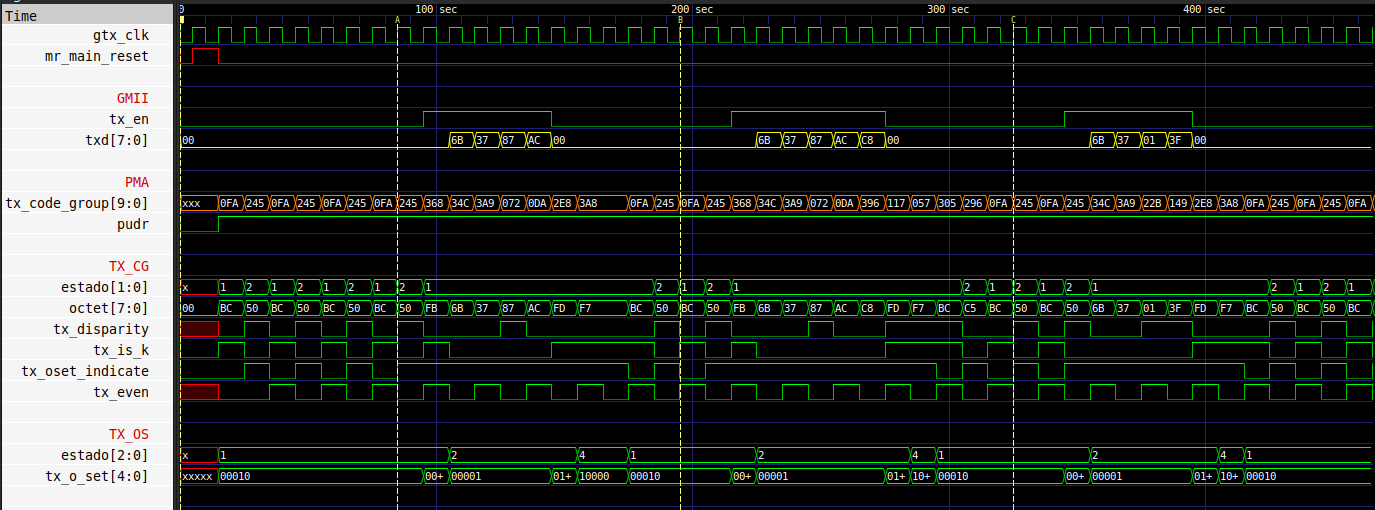
\includegraphics[width=\textwidth]{images/pruebas_transmit.png}
    \caption{Ejecución de prueba 0, 1, 2 y 3 para el \texttt{TRANSMIT}.}
    \label{fig:transmit_prueba0y1}
\end{figure}

\subsection{Módulo \texttt{SYNCHRONIZATION}}


Primero, se muestran los resultados para las pruebas 1 y 2.
Se verifica el correcto funcionamiento del módulo a la hora de recibir las \texttt{COMMA} para la sincronización inicial, entrando al estado de \texttt{SYNC\_ACQUIRED\_1}. Las pruebas se pueden observar en la primera parte de la Figura \ref{pruebaSYNC}.
\begin{figure} [H]
    \centering
    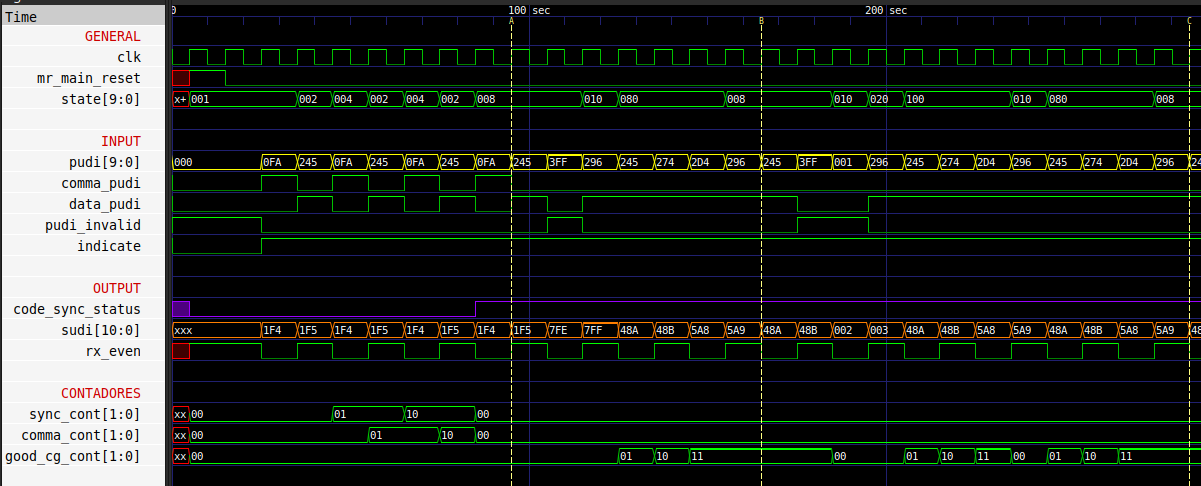
\includegraphics[width=1\linewidth]{images/prueba1_2_y_3_sync.png}
    \caption{Prueba de sincronizaci\'on completa al recibir 3 \textit{comas}}
    \label{pruebaSYNC}
\end{figure}

En la segunda parte de la figura anterior, se ingresa un dato inválido y se vuelve a sincronizar con 4 datos válidos, lo cual cumple exactamente con el comportamiento esperado.
Observe que no se pierde la sincronización completamente (\texttt{code\_sync\_status} = 0), el cual es el comportamiento esperado.

En la Figura \ref{pruebaSYNC2}, se muestran los resultados de las pruebas 5 y 6.
En la prueba 5, se envía un dato inválido y después al intentar volver al estado estable de sincronización, se envía otro.
Por lo tanto, se requiere recibir 8 datos válidos para volver a sincronizarse completamente.
Después de volver al estado \texttt{SYNC\_ACQUIRED\_1}, se realiza la prueba 6, que corresponde a la pérdida de sincronización completa.
Para ello, se envían 4 code-groups inválidos y se transiciona al estado \texttt{LOSS\_OF\_SYNC}.
Para el sincronizador, también se concluye que las pruebas realizadas fueron exitosas y se determinó su funcionamiento correcto según el estándar.

\begin{figure} [H]
    \centering
    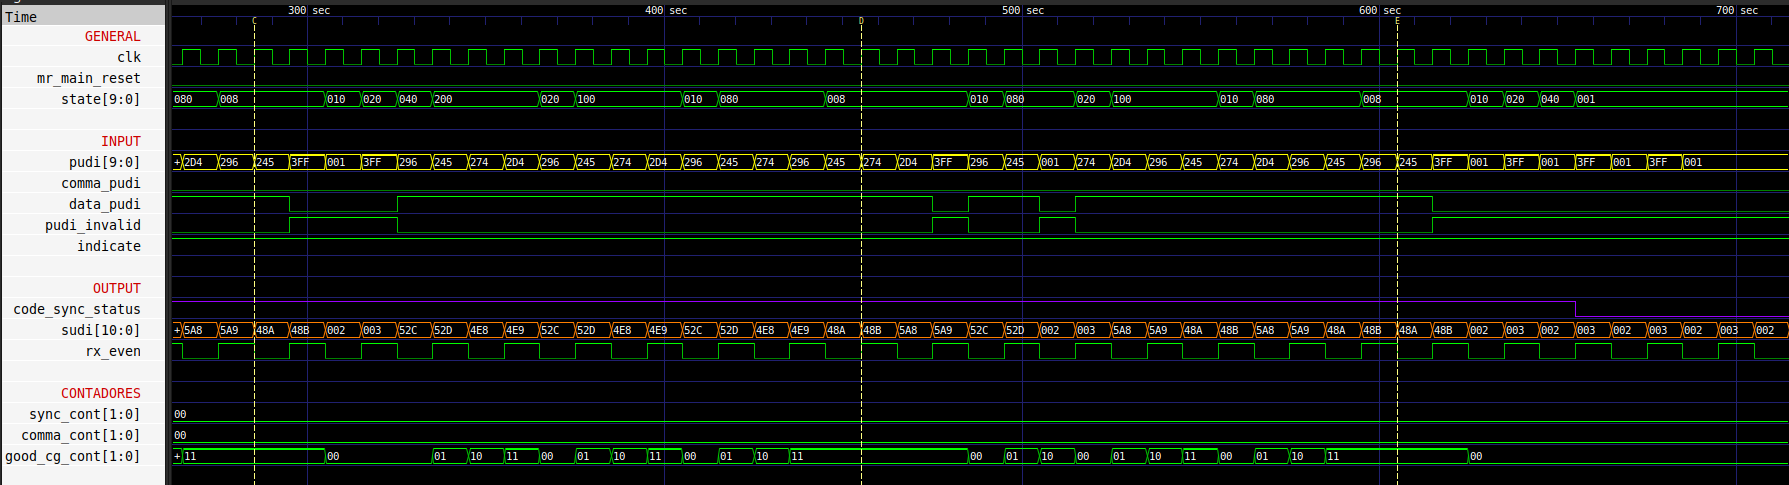
\includegraphics[width=1\linewidth]{images/prueba4_5_y_6_sync.png}
    \caption{Prueba al recibir datos err\'oneos}
    \label{pruebaSYNC2}
\end{figure}


\subsection{Módulo \texttt{RECEIVE}}

Los resultados del módulo \texttt{RECEIVE} se muestran a continuación.

\subsubsection{Envío de datos}
\begin{figure}[H]
    \centering
    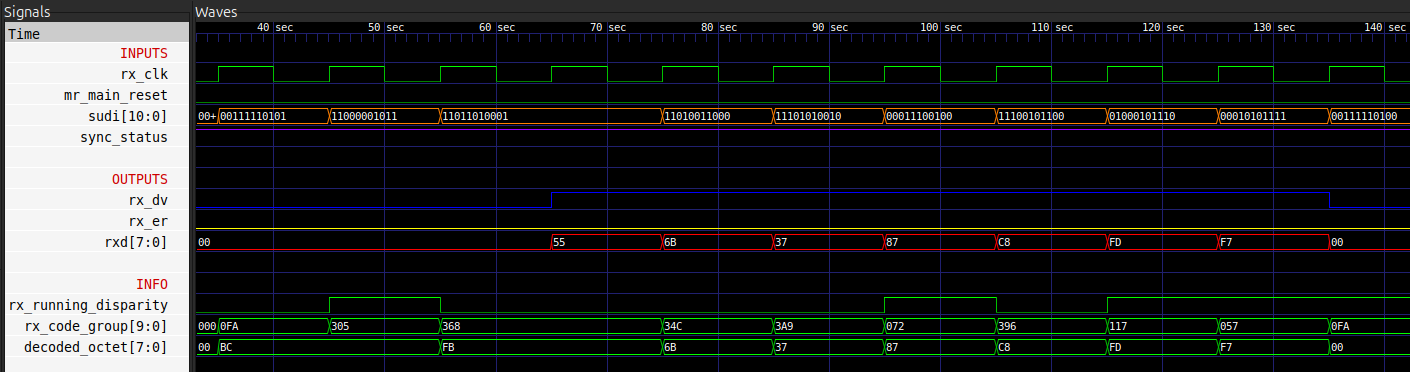
\includegraphics[width=0.9\linewidth]{images/prueba1_receive.png}
    \caption{Resultados obtenidos en la prueba de envío de datos.}
    \label{fig_prueba1_receive}
\end{figure}
\indent En la Figura \ref{fig_prueba1_receive} se puede observar los resultados obtenidos luego del envío de datos, en la señal de color naranja se puede observar la entrada SUDI, la cual trae consigo el rx code group, se puede observar que cuando se recibe la señal de start se activa la salida \texttt{rx\_dv}, la cual es la señal de color azul, y se envía a través de la señal rxd, la cual está de color rojo, un valor de 55, el cual viene mencionado en el estándar que se debe de enviar en el estado de start, seguido a esto se reciben los datos que se mencionaron en el Cuadro \ref{prueba1_receive} y se puede observar que rxd está enviando de manera correcta el octeto específico. Así también cuando se envía un T/R/I deja de enviar datos, ya que esto significa que ya se ha concluido el envío de datos.

\subsubsection{Envío de datos, pero el receptor no está sincronizado}
\indent Al realizar esta prueba se obtuvieron los resultados esperados, por lo que se concluye que el receptor no fallaría si se le presenta esta situación.

\subsubsection{Terminación /T/R/R/}
\indent Al realizar esta prueba los resultados fueron los esperados, ya que efectivamente el receptor detectó la secuencia /T/R/R y en el siguiente ciclo de reloj se activó la señal rx er y rxd tomó el valor de 0x0F y seguidamente terminó el envío de datos.

\subsection{PCS completa}

En cuanto a los resultados aplicados a la PCS completa, se determinaron satisfactorios y se obtuvo el resultado esperado.
Las pruebas realizadas son similares a las aplicadas en el módulo de \texttt{TRANSMIT} individualmente.

En la Figura \ref{fig_prueba_1_pcs}, se muestra inicialmente la sincronización en el primer bloque, donde se reciben caracteres /K28.5/ y finalmente se activa \texttt{code\_sync\_status}.
Luego, se realiza el envío de una trama que tiene que aplicar \textit{carrier extend}. Se observa que efectivamente tiene un envío correcto de esta y la decodificación es exitosa en \texttt{rxd}.
En la tercera prueba de la figura, se envía una trama que no requiere \textit{carrier extend}.
Por lo tanto, estos resultados fueron los esperados para la prueba 0, 1 y 2.

\begin{figure}[H]
    \centering
    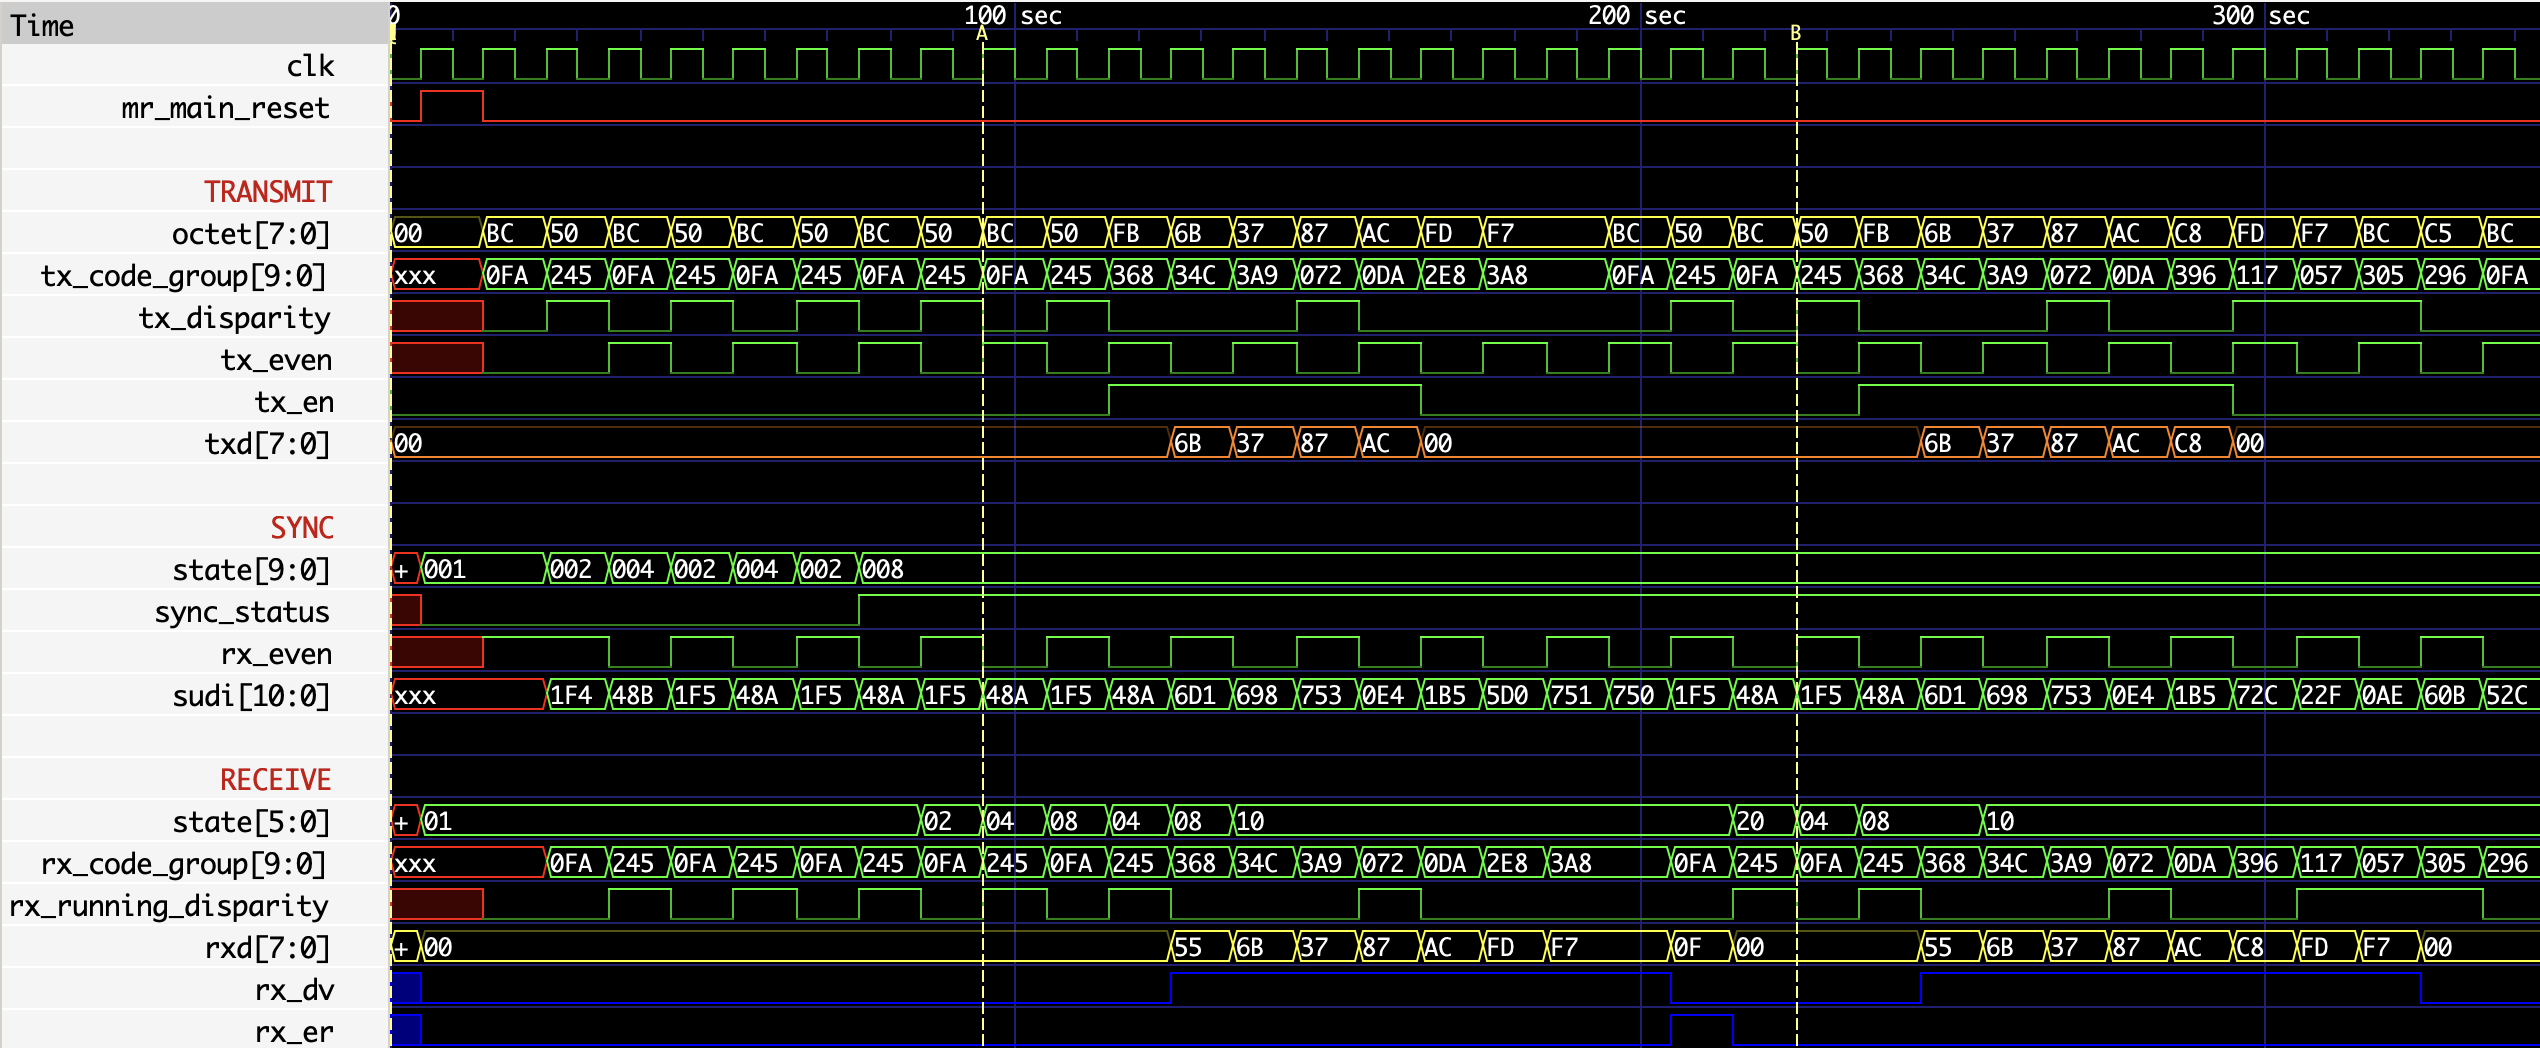
\includegraphics[width=\linewidth]{images/pruebas_pcs_1.png}
    \caption{Prueba de sincronización, envío de trama con \textit{carrier extend} y sin \textit{carrier extend}.}
    \label{fig_prueba_1_pcs}
\end{figure}

Luego, en la Figura \ref{fig_prueba_2_pcs}, se realiza el envío de todos los code-groups que fueron seleccionados (prueba 4), para verificar su correcta codificación y decodificación.
En la prueba 5, mostrada al final de la imagen, se envían los code-groups inválidos descritos en la sección del plan de pruebas y se observa que se pierde la sincronía después de 4 inválidos.
Acá, \texttt{rxd} está en bajo y \texttt{rx\_dv} está en bajo.

\begin{figure}[H]
    \centering
    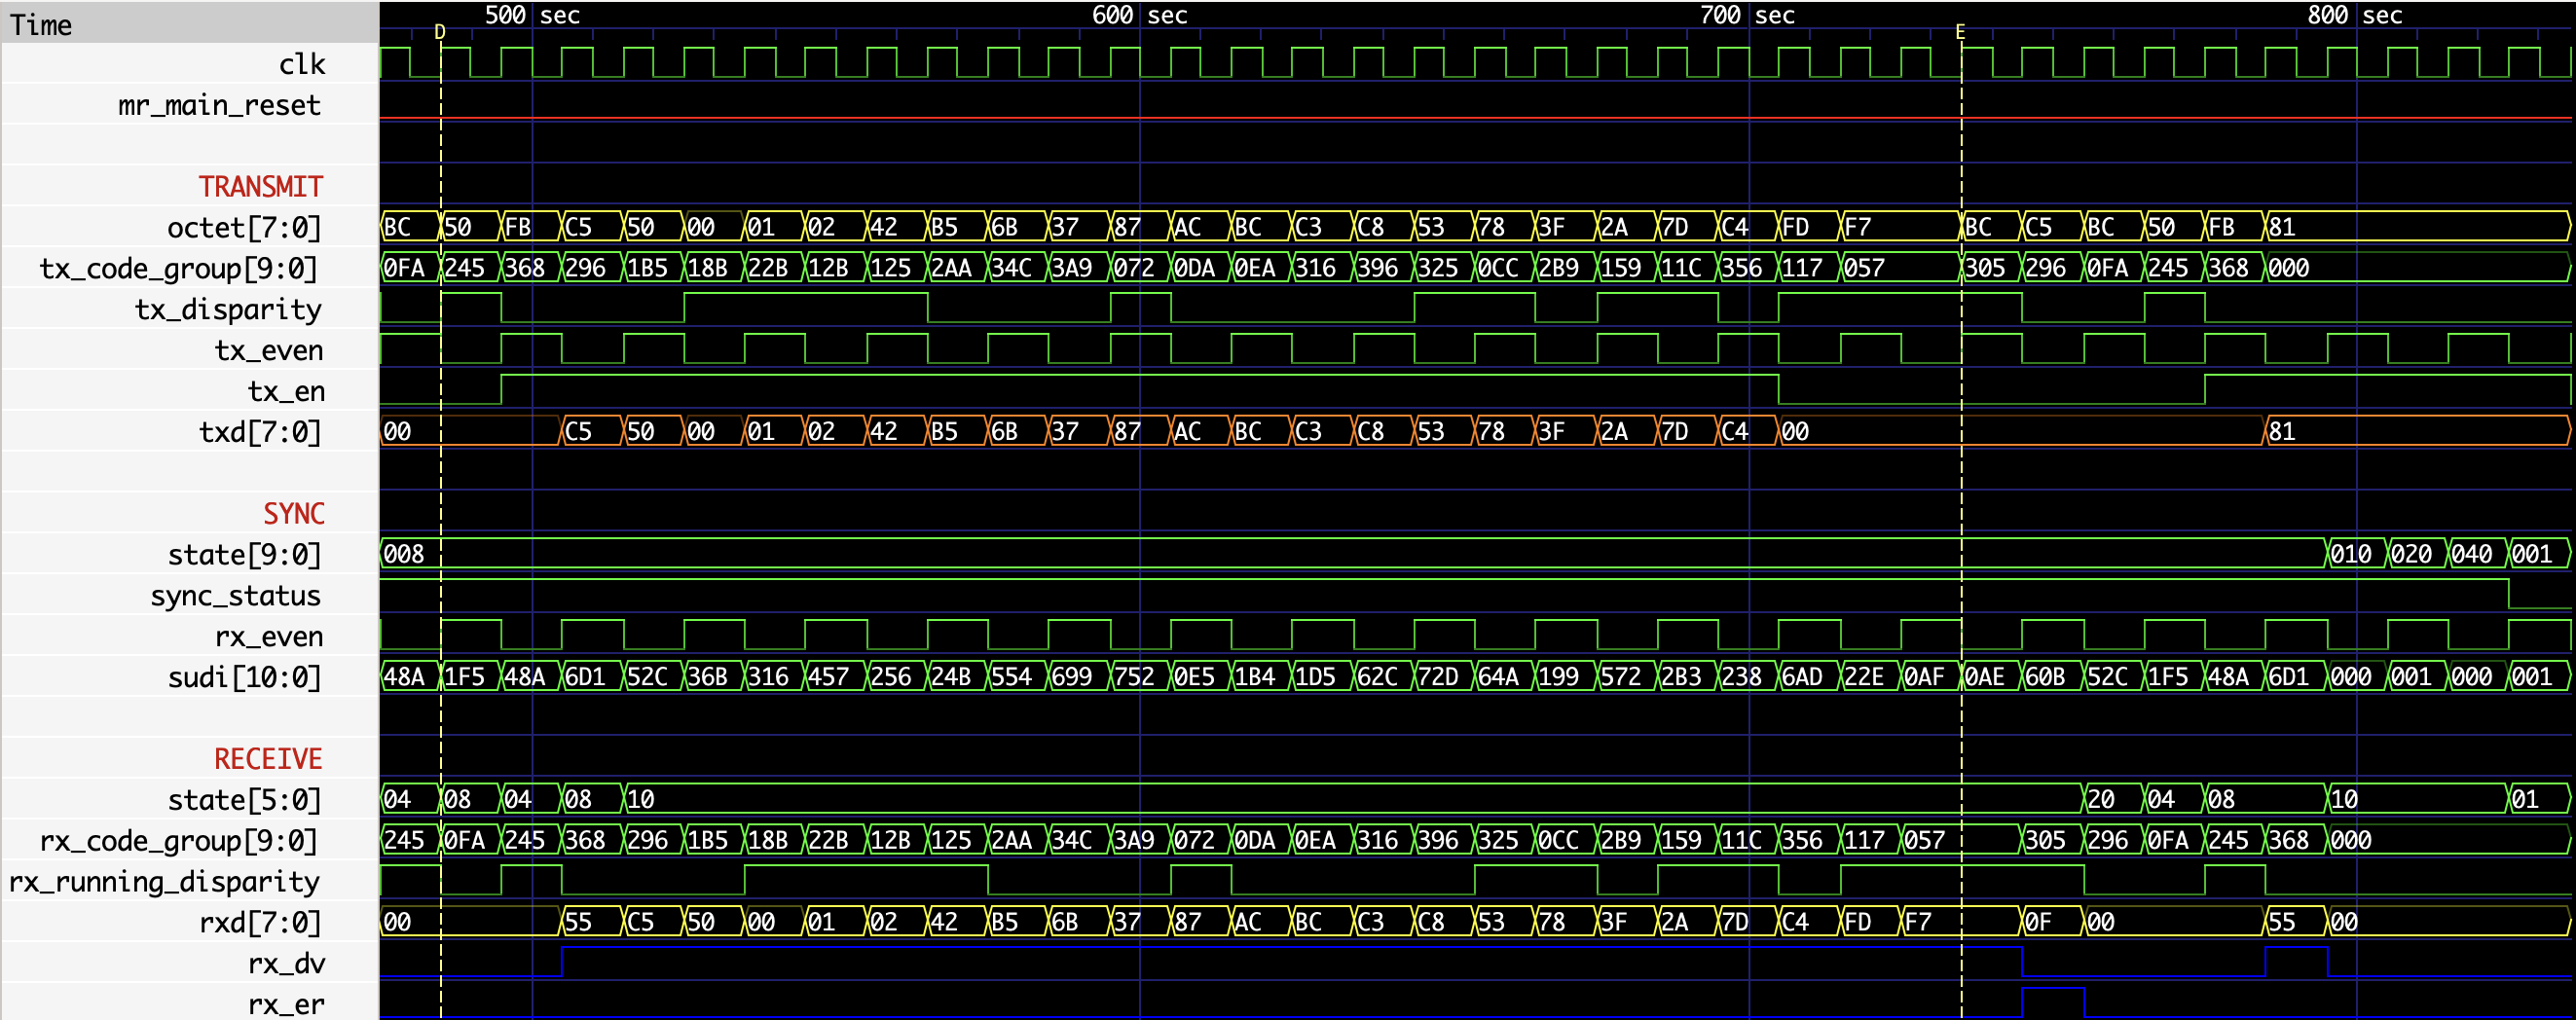
\includegraphics[width=\linewidth]{images/pruebas_pcs_2.png}
    \caption{Prueba de envío de todos los code-groups seleccionados y pérdida de sincronía.}
    \label{fig_prueba_2_pcs}
\end{figure}
\section{Conclusiones y recomendaciones}

En primer lugar, respecto a las conclusiones del proyecto realizado, estas se enumeran a continuación:

\begin{itemize}
    \item Se logró una comprensión sólida de la cláusula 36 del estándar IEEE~802.3, lo cual permitió definir el comportamiento esperado de la PCS y de cada uno de los módulos desarrollados.
    \item Se consiguió una implementación adecuada con el funcionamiento esperado de uno de los módulos de interés que integran la PCS, así como un resultado satisfactorio para la integración de los tres.
    \item El plan de pruebas desarrollado permitió asegurar el funcionamiento, tanto en el caso idóneo como en algunos casos de error (especialmente en el caso del sincronizador). De esta forma, la integración de los tres resultó más sencilla, pues ya se conocía el comportamiento individual de los módulos.
    \item El uso de un enfoque modular resultó adecuado y eficiente, permitiendo que cada integrante del grupo trabajara en un bloque independiente sin comprometer la coherencia del diseño total.
    \item La adopción de convenciones unificadas en nombres de señales, estilos de codificación y estructura de archivos facilitó considerablemente la revisión del código y la colaboración entre los participantes.
    \item El repositorio y flujo de trabajo en GitHub favorecieron una gestión ordenada del proyecto, evitando conflictos y permitiendo avanzar de manera paralela en diferentes componentes.
\end{itemize}

En cuanto a las recomendaciones para la siguiente etapa del proyecto, se proponen las siguientes:

\begin{itemize}
    \item Realizar la síntesis de los módulos.
    \item Implementar casos de configuración y de error en cada uno de los submódulos para tener un desarrollo completo de la cláusula del estándar.
    \item Explorar la implementación del bloque de Auto-Negotiation y Carrier-Sense para completar la PCS del estándar IEEE 802.3.
\end{itemize}



% ----------------------------- %
% References:  BibTeX
% ----------------------------- %
\bibliography{refs.bib}
\bibliographystyle{IEEEtran}


\end{document}
